% ============================================================================
% AI for Business & Economic Research: From Chatbots to Agents
%   Master Class — Penn State Smeal College of Business
% ============================================================================
\documentclass[aspectratio=169, 11pt]{beamer}

% =============================================================================
% THEME: Minimal and Clean (Metropolis-inspired without requiring the package)
% =============================================================================
\usetheme{default}
\usecolortheme{default}

% ---------- colour palette (4 colours, matching Baylor style) ----------------
\definecolor{darkblue}{RGB}{0,51,102}
\definecolor{lightgray}{RGB}{245,245,245}
\definecolor{medgray}{RGB}{100,100,100}
\definecolor{accentorange}{RGB}{230,126,34}

% Legacy aliases (so existing TikZ code compiles without mass-renaming)
\colorlet{navy}{darkblue}
\colorlet{deepnavy}{darkblue}
\colorlet{gold}{accentorange}
\colorlet{warmgold}{accentorange}
\colorlet{coral}{red!70}
\colorlet{sage}{green!60!black}
\colorlet{slate}{medgray}
\colorlet{iceblue}{darkblue!30}
\colorlet{lightice}{lightgray}
\colorlet{offwhite}{white}
\colorlet{midgray}{medgray}
\colorlet{codebg}{lightgray}
\colorlet{codetext}{black}

% ---------- beamer theme settings --------------------------------------------
\setbeamercolor{frametitle}{fg=darkblue, bg=white}
\setbeamercolor{title}{fg=darkblue}
\setbeamercolor{subtitle}{fg=medgray}
\setbeamercolor{structure}{fg=darkblue}
\setbeamercolor{normal text}{fg=black, bg=white}
\setbeamercolor{item}{fg=darkblue}
\setbeamercolor{block title}{fg=white, bg=darkblue}
\setbeamercolor{block body}{fg=black, bg=lightgray}
\setbeamercolor{alerted text}{fg=accentorange}
\setbeamercolor{section in toc}{fg=darkblue}
\setbeamercolor{section number projected}{bg=darkblue, fg=white}
\setbeamertemplate{section in toc}[sections numbered]
\setbeamertemplate{navigation symbols}{}

% ---------- fonts ------------------------------------------------------------
\usefonttheme{professionalfonts}
\setbeamerfont{title}{size=\LARGE, series=\bfseries}
\setbeamerfont{frametitle}{size=\large, series=\bfseries}

% ---------- packages ---------------------------------------------------------
\usepackage[T1]{fontenc}
\usepackage{lmodern}
\usepackage{microtype}
\usepackage{tikz}
\usetikzlibrary{calc, positioning, arrows.meta, shapes.geometric,
                 shapes.symbols, fit, backgrounds, decorations.pathreplacing}
\usepackage{tcolorbox}
\tcbuselibrary{skins, breakable}
\usepackage{booktabs}
\usepackage{graphicx}
\usepackage{xurl}
\usepackage{hyperref}
\usepackage{adjustbox}
\usepackage{etoolbox}
\usepackage{ragged2e}
\usepackage{listings}
\usepackage{amsmath,amssymb}
\usepackage{soul}

% ---------- Global TikZ styles -----------------------------------------------
\tikzset{
  auditbase/.style={draw=none, rounded corners=4pt,
    text width=2.6cm, minimum height=3.3cm, inner sep=6pt, align=center},
  auditlabel/.style={font=\footnotesize\bfseries, text=white},
  audittext/.style={font=\scriptsize, text width=2.3cm, align=left},
  agentbase/.style={draw=none, rounded corners=4pt,
    text width=3.5cm, minimum height=3.0cm, inner sep=6pt, align=center},
  agentlabel/.style={font=\footnotesize\bfseries, text=white},
  agenttext/.style={font=\scriptsize, text width=3.0cm, align=left},
  phasebase/.style={draw=none, rounded corners=4pt,
    text width=2.6cm, minimum height=2.8cm, inner sep=6pt, align=center},
  phaselabel/.style={font=\footnotesize\bfseries, text=white},
  phasetext/.style={font=\scriptsize, text width=2.3cm, align=left},
}

% ---------- safer defaults for graphics -------------------------------------
\setkeys{Gin}{width=\linewidth,height=0.75\textheight,keepaspectratio}

% ---------- Frame title: dark blue text + thin rule --------------------------
\setbeamertemplate{frametitle}{%
  \vspace{0.35cm}%
  \insertframetitle%
  \vspace{0.15cm}%
  \hrule height 0.5pt%
  \vspace{0.25cm}%
}

% ---------- Footer: right-aligned page numbers only --------------------------
\setbeamertemplate{footline}{%
  \hfill\scriptsize\insertframenumber/\inserttotalframenumber\hspace{0.5cm}\vspace{0.3cm}%
}

% ---------- Section break slides ---------------------------------------------
\AtBeginSection[]{%
  \begin{frame}[plain]
  \vfill
  \begin{center}
    {\Large\bfseries\textcolor{darkblue}{\insertsectionnumber}}\\[0.3cm]
    {\LARGE\bfseries\textcolor{darkblue}{\insertsection}}
  \end{center}
  \vfill
  \end{frame}
}

\AtBeginEnvironment{frame}{%
  \setlength{\emergencystretch}{2em}%
}

% ---------- Code listing style -----------------------------------------------
\lstset{
  basicstyle=\ttfamily\scriptsize,
  backgroundcolor=\color{lightgray},
  frame=single, framerule=0pt,
  breaklines=true
}

% ---------- tcolorbox styles -------------------------------------------------
\newtcolorbox{keyinsight}[1][]{%
  enhanced,
  colback=lightgray, colframe=lightgray, boxrule=0pt,
  borderline north={1.5pt}{0pt}{darkblue},
  sharp corners, left=8pt, right=8pt, top=6pt, bottom=6pt,
  fonttitle=\bfseries\color{white},
  coltitle=white, colbacktitle=darkblue,
  title={#1}
}
\newtcolorbox{quotebox}{%
  enhanced,
  colback=lightgray, colframe=lightgray, boxrule=0pt,
  sharp corners, left=8pt, right=8pt, top=6pt, bottom=6pt,
}
\newtcolorbox{warningbox}[1][]{%
  enhanced,
  colback=lightgray, colframe=lightgray, boxrule=0pt,
  borderline north={1.5pt}{0pt}{darkblue},
  sharp corners, left=8pt, right=8pt, top=6pt, bottom=6pt,
  fonttitle=\bfseries\color{white},
  coltitle=white, colbacktitle=darkblue,
  title={#1}
}
\newtcolorbox{codeblock}{%
  enhanced,
  colback=lightgray, colframe=lightgray, sharp corners,
  left=8pt, right=8pt, top=6pt, bottom=6pt, boxrule=0pt,
  width=\linewidth
}

% ---------- quote slide box (orange left border) -----------------------------
\newtcolorbox{bigquote}{%
  enhanced,
  colback=lightgray, colframe=lightgray, boxrule=0pt,
  borderline west={3pt}{0pt}{accentorange},
  sharp corners, left=12pt, right=12pt, top=10pt, bottom=10pt,
}

% ---------- custom commands --------------------------------------------------
\newcommand{\emphgold}[1]{\alert{\textbf{#1}}}
\newcommand{\emphcoral}[1]{\textcolor{red}{\textbf{#1}}}
\newcommand{\emphsage}[1]{\textcolor{green!60!black}{\textbf{#1}}}
\newcommand{\emphslate}[1]{\textcolor{medgray}{#1}}
\newcommand{\cmark}{\textcolor{accentorange}{\texttt{>}}\;\,}
\newcommand{\codett}[1]{{\ttfamily\scriptsize\raggedright\hyphenpenalty=50\exhyphenpenalty=50 #1}}
\newcommand{\sourceref}[1]{\vspace{0.15cm}\hfill{\tiny\textcolor{medgray}{#1}}}

% =============================================================================
% DOCUMENT
% =============================================================================
\title{AI for Business \& Economic Research}
\subtitle{From Chatbots to Agents}
\author{Mihail Velikov}
\institute{Penn State --- Smeal College of Business}
\date{AI Community of Practice in Research\\ April 6, 2026}

\begin{document}

% ---------- Title slide ------------------------------------------------------
\begin{frame}[plain]
\titlepage
\end{frame}

% ---------- Outline ----------------------------------------------------------
\begin{frame}{Outline}
\tableofcontents
\end{frame}

% =============================================================================
\section{Voices from the Field}
% =============================================================================

% --- Slide 0: Baker — tongue-in-cheek opener ---------------------------------
\begin{frame}{Caveat Emptor}
\vfill
\begin{bigquote}
\Large
``Every morning I wake up and think: do you know what we need more of? \emphgold{Economists talking to us about AI} and what it's going to do to research.''
\end{bigquote}
\vspace{0.5cm}
\hfill\textcolor{medgray}{\normalsize --- Andrew Baker, UC Berkeley Law}
\sourceref{\href{https://www.linkedin.com/posts/andrew-baker-09bb6326_every-morning-i-wake-up-and-think-do-you-activity-7442585905145520128-1xy9}{LinkedIn post}}
\vfill
\end{frame}

% --- Timeline 1: Novy-Marx & Velikov (2024) -----------------------------------
\begin{frame}{2024: Mass Production}
\vfill
\begin{bigquote}
\large
``This study represents an early exploration of AI’s capabilities in producing academic finance research at scale. The tools and methods demonstrated here are in their infancy, and we expect significant advances in the coming years.''
\end{bigquote}
\vspace{0.5cm}
\hfill\textcolor{medgray}{\normalsize --- Novy-Marx \& Velikov (2026)}
\sourceref{\href{https://papers.ssrn.com/sol3/papers.cfm?abstract_id=5060022}{SSRN} · \href{https://github.com/velikov-mihail/AI-Powered-Scholarship}{GitHub}}
\vfill
\end{frame}

% --- Timeline 2: Andrew Chen (2025) -------------------------------------------
\begin{frame}{Early 2025: AI as Junior Co-Author}
\vfill
\begin{bigquote}
\large
``I had been repeatedly shocked by AI progress. I was using AI to prove theorems, vibe coding, and AI lit reviews in my daily life. Six months ago, I had thought each of these things is impossible. What will happen in the next six years?! Will my entire job be replaced by AI? \emphgold{I have no idea.}''
\end{bigquote}
\vspace{0.5cm}
\hfill\textcolor{medgray}{\normalsize --- Andrew Chen, Federal Reserve Board}
\sourceref{\href{https://github.com/chenandrewy/Prompts-to-Paper}{GitHub: Prompts-to-Paper}}
\vfill
\end{frame}

% --- Timeline 3: Joshua Gans (2025) ------------------------------------------
\begin{frame}{Full Year 2025: AI-First Research}
\vfill
\begin{bigquote}
\large
``If you look at my website, 2025 produced \emphgold{a lot of working papers}. A few have been accepted for publication\ldots\ A few others are R\&R at better journals. I haven't yet broken through at a top-tier journal, but I did fail at a number.''
\end{bigquote}
\vspace{0.5cm}
\hfill\textcolor{medgray}{\normalsize --- Joshua Gans, ``Reflections on Vibe Researching'' (2026)}
\sourceref{\href{https://joshuagans.substack.com/p/reflections-on-vibe-researching}{Substack}}
\vfill
\end{frame}

% --- Timeline 4: Vincent Gregoire (Feb 2026) ----------------------------------
\begin{frame}{February 2026: Four Days to SSRN}
\vfill
\begin{bigquote}
\Large
``I tried to write an academic paper in four weeks using AI\ldots\ and \emphgold{finished in four days.}''
\end{bigquote}
\vspace{0.5cm}
\hfill\textcolor{medgray}{\normalsize --- Vincent Gregoire, HEC Montreal}
\sourceref{\href{https://vincent.codes.finance/posts/vibe-research-paper/}{Blog post}}
\vfill
\end{frame}

% --- Timeline 5: Paul Novosad (2026) ------------------------------------------
\begin{frame}{2026: The 3-Hour Paper}
\vfill
\begin{bigquote}
\Large
``I wrote a decent paper with AI. It took me about \emphgold{3 hours} from start to finish, including an interactive choose-your-own-border RD adventure. It's a \emphgold{what are we even doing here} kind of day.''
\end{bigquote}
\vspace{0.5cm}
\hfill\textcolor{medgray}{\normalsize --- Paul Novosad, Dartmouth}
\sourceref{\href{https://x.com/paulnovosad/status/2021655122351468684}{X post}}
\vfill
\end{frame}

% --- Timeline 6: Project APE (March 2026) -------------------------------------
\begin{frame}{March 2026: Zero Human Involvement}
\vfill
\begin{bigquote}
\large
``Claude Code drives the \emphgold{entire pipeline}: generating research ideas, writing R scripts, fetching data, running analysis, drafting \LaTeX, and revising based on feedback. It operates as an agentic coding system --- planning, executing, and iterating autonomously.''
\end{bigquote}
\vspace{0.5cm}
\hfill\textcolor{medgray}{\normalsize --- Project APE}
\sourceref{\href{https://ape.socialcatalystlab.org/methodology}{ape.socialcatalystlab.org}}
\vspace{0.3cm}
\begin{center}
\large
\textbf{The arc:} Years $\rightarrow$ Weeks $\rightarrow$ Days $\rightarrow$ Hours $\rightarrow$ \emphgold{Zero}
\end{center}
\vfill
\end{frame}

% --- Beyond research: coding and math ------------------------------------------
\begin{frame}{Meanwhile, Outside Economics\ldots}
\begin{tcolorbox}[enhanced, colback=lightgray, colframe=lightgray, boxrule=0pt,
  borderline west={3pt}{0pt}{accentorange}, sharp corners,
  left=8pt, right=8pt, top=3pt, bottom=3pt]
\footnotesize
``AI is now writing \emphgold{much of the code} at Anthropic\ldots\ We may be only \emphgold{1--2 years away} from a point where the current generation of AI autonomously builds the next.''
\end{tcolorbox}
\vspace{-0.2cm}
\hfill\textcolor{medgray}{\scriptsize --- Dario Amodei, CEO of Anthropic\quad\href{https://www.dwarkeshpatel.com/p/dario-amodei}{Dwarkesh Podcast}}
\vspace{-0.1cm}
\begin{tcolorbox}[enhanced, colback=lightgray, colframe=lightgray, boxrule=0pt,
  borderline west={3pt}{0pt}{accentorange}, sharp corners,
  left=8pt, right=8pt, top=3pt, bottom=3pt]
\footnotesize
``GPT-5.3-Codex is our first model that was \emphgold{instrumental in creating itself}.''
\end{tcolorbox}
\vspace{-0.2cm}
\hfill\textcolor{medgray}{\scriptsize --- \href{https://openai.com/index/introducing-gpt-5-3-codex/}{OpenAI} (2026)}
\vspace{-0.1cm}
\begin{tcolorbox}[enhanced, colback=lightgray, colframe=lightgray, boxrule=0pt,
  borderline west={3pt}{0pt}{accentorange}, sharp corners,
  left=8pt, right=8pt, top=3pt, bottom=3pt]
\footnotesize
``An Erd\H{o}s problem (\#728) was solved \emphgold{more or less autonomously by AI}\ldots\ with the result not replicated in existing literature.''
\end{tcolorbox}
\vspace{-0.2cm}
\hfill\textcolor{medgray}{\scriptsize --- Terence Tao, Fields Medalist\quad\href{https://mathstodon.xyz/@tao/115855840223258103}{Mastodon post}}
\vspace{-0.1cm}
\begin{tcolorbox}[enhanced, colback=lightgray, colframe=lightgray, boxrule=0pt,
  borderline west={3pt}{0pt}{accentorange}, sharp corners,
  left=8pt, right=8pt, top=3pt, bottom=3pt]
\footnotesize
In July 2025, AI earned \emphgold{gold medals} at the International Mathematical Olympiad --- three teams, three different approaches.
\end{tcolorbox}
\vspace{-0.2cm}
\hfill\textcolor{medgray}{\scriptsize\href{https://deepmind.google/blog/advanced-version-of-gemini-with-deep-think-officially-achieves-gold-medal-standard-at-the-international-mathematical-olympiad/}{Google DeepMind blog}}
\end{frame}

% =============================================================================
\section{Evolution of AI}
% =============================================================================

% --- Slide 11: Three paradigms overview ---------------------------------------
\begin{frame}[shrink=7]{Three Paradigms of Generative AI}
\begin{center}
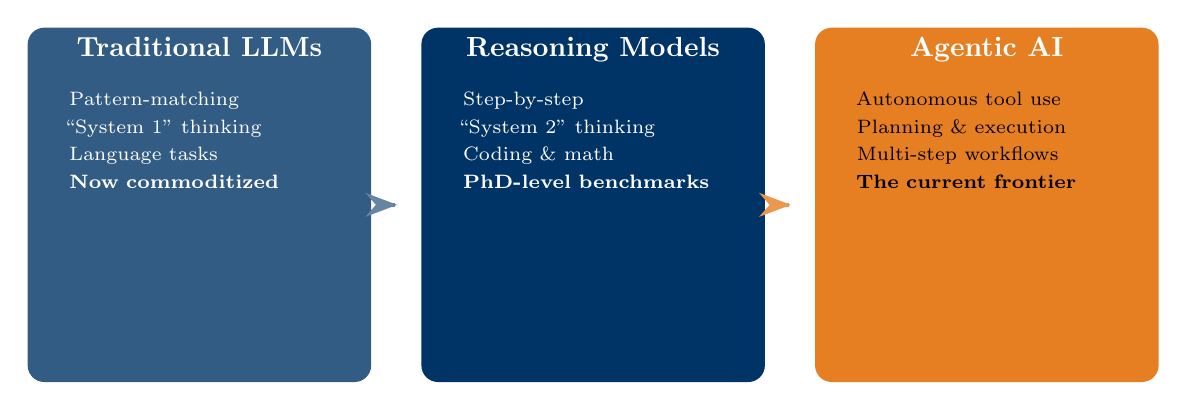
\begin{tikzpicture}[
  paradigm/.style={draw=none, rounded corners=6pt, text width=3.8cm,
    minimum height=4.5cm, inner sep=8pt, align=center},
  plabel/.style={font=\normalsize\bfseries, text=white},
  ptext/.style={font=\scriptsize, text width=3.3cm, align=left},
]
% Column 1: Traditional LLMs
\node[paradigm, fill=darkblue!80] (llm) at (0,0) {};
\node[plabel, anchor=north] at (llm.north) {Traditional LLMs};
\node[ptext, anchor=north, text=white] at ([yshift=-0.7cm]llm.north) {%
  Pattern-matching\\[2pt]
  ``System 1'' thinking\\[2pt]
  Language tasks\\[2pt]
  \textbf{Now commoditized}
};

% Column 2: Reasoning Models
\node[paradigm, fill=darkblue] (reason) at (5,0) {};
\node[plabel, anchor=north] at (reason.north) {Reasoning Models};
\node[ptext, anchor=north, text=white] at ([yshift=-0.7cm]reason.north) {%
  Step-by-step\\[2pt]
  ``System 2'' thinking\\[2pt]
  Coding \& math\\[2pt]
  \textbf{PhD-level benchmarks}
};

% Column 3: Agentic AI
\node[paradigm, fill=accentorange] (agent) at (10,0) {};
\node[plabel, anchor=north] at (agent.north) {Agentic AI};
\node[ptext, anchor=north] at ([yshift=-0.7cm]agent.north) {%
  Autonomous tool use\\[2pt]
  Planning \& execution\\[2pt]
  Multi-step workflows\\[2pt]
  \textbf{The current frontier}
};

% Arrows
\draw[-{Stealth[length=4mm]}, line width=1.5pt, darkblue!60]
  ([xshift=3mm]llm.east) -- ([xshift=-3mm]reason.west);
\draw[-{Stealth[length=4mm]}, line width=1.5pt, accentorange!80]
  ([xshift=3mm]reason.east) -- ([xshift=-3mm]agent.west);
\end{tikzpicture}
\end{center}
\vspace{0.1cm}
\begin{center}
\small\textcolor{medgray}{Amodei: AI models ``substantially smarter than almost all humans at almost all tasks'' on track for 2026--27.}
\end{center}
\sourceref{Korinek (2025), ``Generative AI for Economic Research'' -- JEL update}
\end{frame}

% --- Traditional LLMs — commoditized -----------------------------------------
\begin{frame}{Paradigm 1: Traditional LLMs}
\begin{columns}[T]
\column{0.55\textwidth}
\begin{itemize}
  \item Single-pass text generation (``System 1'')
  \item Dominant for: writing, summarization, translation, brainstorming
  \item ChatGPT Instant 5.3, Claude Sonnet 4.6, Gemini 3 Flash, Llama 4, Qwen3
\end{itemize}
\vspace{0.5cm}
\begin{keyinsight}[Key Takeaway]
LLM capabilities are now \emphgold{commoditized} --- differentiation has shifted to reasoning and agentic capabilities.
\end{keyinsight}

\column{0.40\textwidth}
\begin{center}
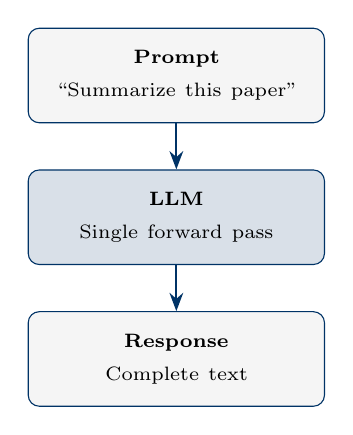
\begin{tikzpicture}[scale=0.9]
  \node[draw=darkblue, rounded corners, fill=lightgray,
        text width=3.2cm, align=center, inner sep=8pt] (input) at (0,2)
    {\scriptsize\textbf{Prompt}\\``Summarize this paper''};
  \node[draw=darkblue, rounded corners, fill=darkblue!15,
        text width=3.2cm, align=center, inner sep=8pt] (llm) at (0,0)
    {\scriptsize\textbf{LLM}\\Single forward pass};
  \node[draw=darkblue, rounded corners, fill=lightgray,
        text width=3.2cm, align=center, inner sep=8pt] (output) at (0,-2)
    {\scriptsize\textbf{Response}\\Complete text};
  \draw[-{Stealth}, thick, darkblue] (input) -- (llm);
  \draw[-{Stealth}, thick, darkblue] (llm) -- (output);
\end{tikzpicture}
\end{center}
\end{columns}
\end{frame}

% --- Slide 13: Reasoning models — benchmarks ----------------------------------
\begin{frame}[shrink=1]{Paradigm 2: Reasoning Models}
\begin{columns}[T]
\column{0.55\textwidth}
\begin{itemize}
  \item Chain-of-thought, step-by-step reasoning (``System 2'')
  \item Trained via reinforcement learning to ``think before answering''
  \item ChatGPT Thinking 5.4, Claude Opus 4.6, Gemini 3.1 Pro, Grok-4 Heavy
\end{itemize}
\vspace{0.3cm}
\begin{keyinsight}[PhD-Level Performance]
These models now approach or exceed expert-level performance on scientific reasoning benchmarks.
\end{keyinsight}

\column{0.42\textwidth}
\begin{center}
\footnotesize
\begin{tabular}{@{}lc@{}}
\toprule
\textbf{Benchmark} & \textbf{Best} \\
\midrule
GPQA (science) & 94.3\% \\
IMO (math) & Gold medal \\
SWE-Bench & $\sim$75\% \\
\bottomrule
\end{tabular}
\end{center}
\vspace{0.4cm}
\begin{center}
\scriptsize\textcolor{medgray}{PhD experts score $\sim$65\% on GPQA}
\end{center}
\end{columns}
\sourceref{\href{https://llm-stats.com/benchmarks/gpqa}{GPQA Leaderboard} (April 2026); Korinek (2025)}
\end{frame}

% --- Frontier model landscape --------------------------------------------------
\begin{frame}[shrink=10]{The Frontier Model Landscape (March 2026)}
\begin{center}
\footnotesize
\renewcommand{\arraystretch}{1.4}
\begin{tabular}{@{} l c c c @{}}
\toprule
 & \textbf{OpenAI} & \textbf{Anthropic} & \textbf{Google} \\
\midrule
\textbf{Fast / Traditional} & Instant 5.3 & Sonnet 4.6, Haiku 4.5 & Gemini 3 Flash \\[2pt]
\textbf{Reasoning} & Thinking 5.4, Pro & Opus 4.6 & Gemini 3.1 Pro, \\
 & & (Extended Thinking) & Deep Think \\[2pt]
\textbf{Agentic / Coding} & Codex (GPT-5.4) & Claude Code & Gemini CLI, \\
 & & & Antigravity \\
\midrule
\textbf{GPQA} & \emphgold{93.2\%} (Pro) & 91.3\% & \emphgold{94.3\%} \\
\bottomrule
\end{tabular}
\renewcommand{\arraystretch}{1.0}
\end{center}
\vspace{0.2cm}
\begin{center}
\small
PhD experts score $\sim$65\% on GPQA \quad$\cdot$\quad All three labs achieved \emphgold{IMO gold medals}\\[4pt]
Also: \textbf{xAI} Grok-4 Heavy (88.4\%) \quad$\cdot$\quad \textbf{ByteDance} Seed 2.0 (88.9\%) \quad$\cdot$\quad \textbf{Alibaba} Qwen3.6 (90.4\%)
\end{center}
\sourceref{\href{https://llm-stats.com/benchmarks/gpqa}{GPQA Leaderboard} (April 2026); \href{https://www.oneusefulthing.org/p/a-guide-to-which-ai-to-use-in-the}{Mollick (2026)}}
\end{frame}

% --- Slide 15: Exponential progress — METR ------------------------------------
\begin{frame}[shrink=9]{Exponential Progress}
\vfill
\begin{center}
\includegraphics[width=0.9\linewidth, height=0.75\textheight, keepaspectratio]{./images/metr.png}
\end{center}
\vfill
\sourceref{\href{https://metr.org/blog/2026-1-29-time-horizon-1-1}{METR (2026)}; Mollick (2026); Svoronos (2026)}
\end{frame}

% --- Paradigm 3: Agents ------------------------------------------------------
\begin{frame}{Paradigm 3: Agentic AI}
\begin{columns}[T]
\column{0.55\textwidth}
\begin{itemize}
  \item LLM + \textbf{tools} + \textbf{loop} + \textbf{goal}
  \item Agents \emph{act} --- they execute code, search the web, call APIs, read files
  \item Can plan multi-step strategies and adjust on the fly
  \item Spawn sub-agents for parallel work
\end{itemize}
\vspace{0.3cm}
\begin{keyinsight}[Key Shift]
From ``AI that says things'' to \emphgold{``AI that does things''}.
\end{keyinsight}

\column{0.40\textwidth}
\begin{center}
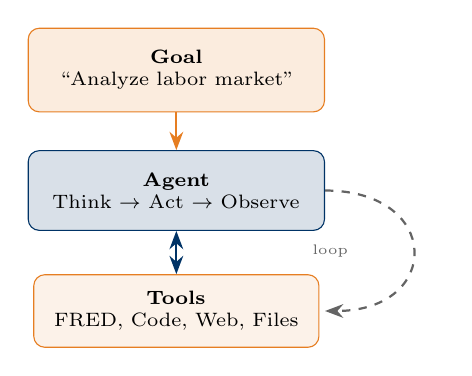
\begin{tikzpicture}[scale=0.85]
  \node[draw=accentorange, rounded corners, fill=accentorange!15,
        text width=3.2cm, align=center, inner sep=8pt, font=\scriptsize]
    (prompt) at (0,3) {\textbf{Goal}\\``Analyze labor market''};
  \node[draw=darkblue, rounded corners, fill=darkblue!15,
        text width=3.2cm, align=center, inner sep=8pt, font=\scriptsize]
    (agent) at (0,1.2) {\textbf{Agent}\\Think $\rightarrow$ Act $\rightarrow$ Observe};
  \node[draw=accentorange, rounded corners, fill=accentorange!10,
        text width=3.2cm, align=center, inner sep=6pt, font=\scriptsize]
    (tools) at (0,-0.6) {\textbf{Tools}\\FRED, Code, Web, Files};
  \draw[-{Stealth}, thick, accentorange] (prompt) -- (agent);
  \draw[{Stealth}-{Stealth}, thick, darkblue] (agent) -- (tools);
  % loop arrow
  \draw[-{Stealth}, thick, medgray, dashed] (agent.east) to[out=0,in=0,looseness=2.5] (agent.east |- tools.east) ;
  \node[font=\tiny, text=medgray] at (2.3,0.3) {loop};
\end{tikzpicture}
\end{center}
\end{columns}
\sourceref{Korinek (2025); Svoronos (2026)}
\end{frame}

% =============================================================================
\section{How an Agent Works}
% =============================================================================

% --- Slide 18: Agent architecture TikZ ----------------------------------------
\begin{frame}[shrink=12]{Agent Architecture}
\begin{center}
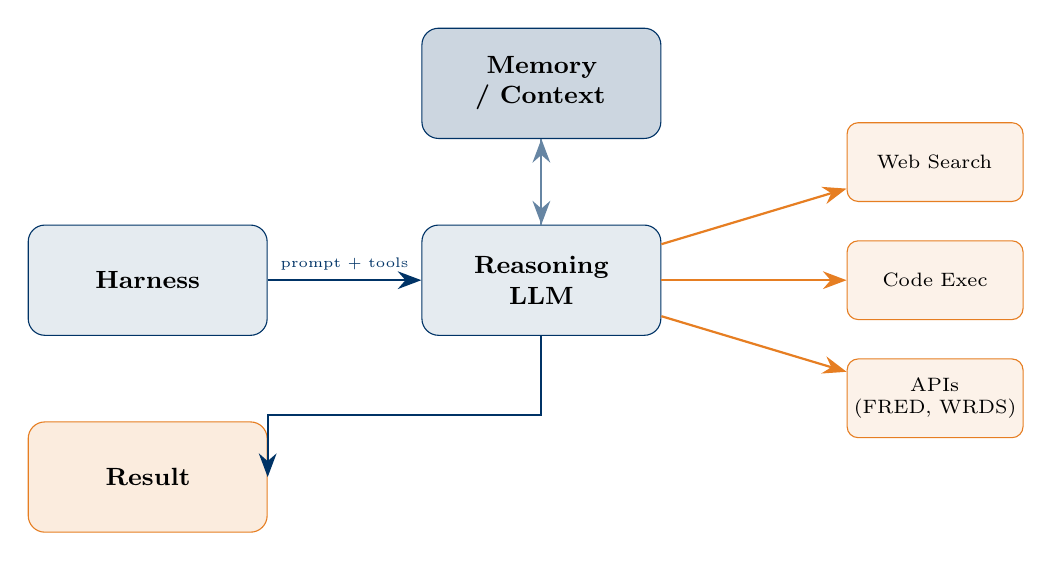
\begin{tikzpicture}[
  block/.style={draw=darkblue, rounded corners=6pt, fill=darkblue!10,
    text width=2.8cm, minimum height=1.4cm, align=center,
    font=\small\bfseries},
  tool/.style={draw=accentorange, rounded corners=4pt, fill=accentorange!10,
    text width=2.0cm, minimum height=1.0cm, align=center,
    font=\scriptsize},
  arw/.style={-{Stealth[length=3mm]}, thick, darkblue},
]
% Main blocks
\node[block] (orch) at (0,0) {Harness};
\node[block] (llm) at (5,0) {Reasoning\\LLM};
\node[block, fill=darkblue!20] (mem) at (5,2.5) {Memory\\/ Context};

% Tools
\node[tool] (search) at (10,1.5) {Web Search};
\node[tool] (code) at (10,0) {Code Exec};
\node[tool] (api) at (10,-1.5) {APIs\\(FRED, WRDS)};

% Result
\node[block, fill=accentorange!15, draw=accentorange] (result) at (0,-2.5)
  {Result};

% Arrows
\draw[arw] (orch) -- node[above, font=\tiny] {prompt + tools} (llm);
\draw[arw, darkblue!60] (llm) -- (mem);
\draw[arw, darkblue!60] (mem) -- (llm);
\draw[arw, accentorange] (llm) -- (search);
\draw[arw, accentorange] (llm) -- (code);
\draw[arw, accentorange] (llm) -- (api);
\draw[arw] (llm.south) -- ++(0,-1) -| (result.east);
\end{tikzpicture}
\end{center}
\sourceref{Korinek (2025)}
\end{frame}

% --- Slide 19: ReAct loop ----------------------------------------------------
\begin{frame}[shrink=10]{The Think--Act--Observe Loop}
\begin{center}
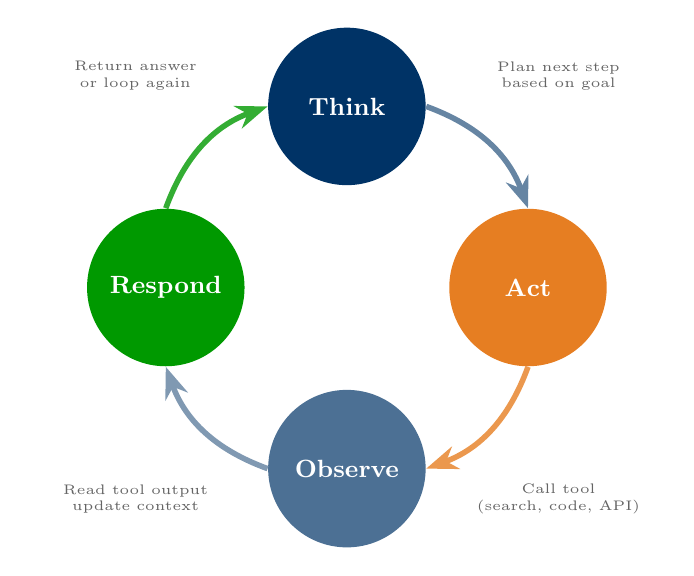
\begin{tikzpicture}[
  phase/.style={draw=none, circle, minimum size=2.0cm, align=center,
    font=\small\bfseries, text=white},
  arw/.style={-{Stealth[length=4mm]}, line width=2pt},
]
% Four phases in a circle
\node[phase, fill=darkblue] (think) at (90:2.3) {Think};
\node[phase, fill=accentorange] (act) at (0:2.3) {Act};
\node[phase, fill=darkblue!70] (obs) at (270:2.3) {Observe};
\node[phase, fill=sage] (resp) at (180:2.3) {Respond};

% Curved arrows
\draw[arw, darkblue!60] (think.east) to[bend left=25] (act.north);
\draw[arw, accentorange!80] (act.south) to[bend left=25] (obs.east);
\draw[arw, darkblue!50] (obs.west) to[bend left=25] (resp.south);
\draw[arw, sage!80] (resp.north) to[bend left=25] (think.west);

% Annotations
\node[font=\tiny, text=medgray, text width=2.5cm, align=center]
  at (45:3.8) {Plan next step\\based on goal};
\node[font=\tiny, text=medgray, text width=2.5cm, align=center]
  at (315:3.8) {Call tool\\(search, code, API)};
\node[font=\tiny, text=medgray, text width=2.5cm, align=center]
  at (225:3.8) {Read tool output\\update context};
\node[font=\tiny, text=medgray, text width=2.5cm, align=center]
  at (135:3.8) {Return answer\\or loop again};
\end{tikzpicture}
\end{center}
\end{frame}

% --- FRED Agent: The Code ------------------------------------------------------
\begin{frame}[fragile,shrink=16]{FRED Agent: The Code}
\begin{columns}[T]
\column{0.52\textwidth}
\begin{lstlisting}[language=Python, basicstyle=\ttfamily\tiny,
  escapeinside={(*@}{@*)}]
class FREDAgent:
  def __init__(self):
    self.fred = Fred(api_key=...)
    self.llm  = OpenAI(api_key=...)

  def think(self, question):
    prompt = "What FRED series code
      answers: " + question
    # LLM returns JSON with code
    return llm_call(prompt)

  def act(self, series_code):
    return self.fred.get_series(
      series_code)

  def observe(self, data, units):
    return dict(value=data.iloc[-1],
                units=units)

  def respond(self, question, obs):
    return llm_call("Answer " +
      question + " using " + obs)

  def answer(self, question):  (*@\textcolor{accentorange}{\# harness}@*)
    code = self.think(question)
    data = self.act(code)
    obs  = self.observe(data)
    return self.respond(question,obs)
\end{lstlisting}

\column{0.44\textwidth}
\vspace{0.3cm}
\begin{itemize}
  \item $\sim$100 lines of Python
  \item The ``intelligence'' is in the \emphgold{prompts} (lines 6--11, 22--23)
  \item Two LLM calls + one API call
  \item Fully \emphgold{vibe-coded}: ``A coding agent wrote this in under a minute'' --- Korinek
\end{itemize}
\vspace{0.3cm}
\begin{keyinsight}[Key Insight]
The agent decides \emph{what} FRED series to fetch based on the question --- it's not a script following predetermined steps.
\end{keyinsight}
\end{columns}
\sourceref{Korinek (2025) --- \href{https://genaiforecon.org}{genaiforecon.org}}
\end{frame}

% --- FRED Agent: In Action -----------------------------------------------------
\begin{frame}[shrink=23]{FRED Agent: In Action}
\begin{keyinsight}[Question: ``What is the US inflation rate?'']
\end{keyinsight}
\vspace{0.2cm}
\begin{center}
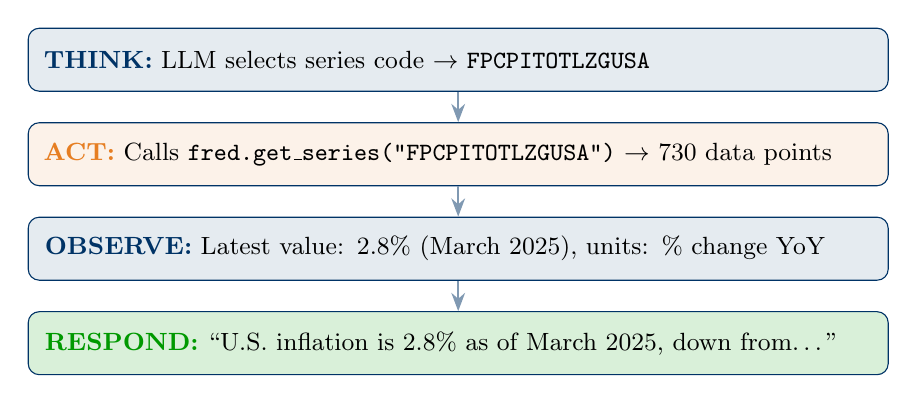
\begin{tikzpicture}[
  stp/.style={draw=darkblue, rounded corners=4pt,
    text width=10.5cm, minimum height=0.8cm, align=left,
    inner sep=6pt, font=\small},
  arw/.style={-{Stealth}, thick, darkblue!50},
]
\node[stp, fill=darkblue!10] (s1) at (0,2.4)
  {\textbf{\textcolor{darkblue}{THINK:}} LLM selects series code $\rightarrow$ \texttt{FPCPITOTLZGUSA}};
\node[stp, fill=accentorange!10] (s2) at (0,1.2)
  {\textbf{\textcolor{accentorange}{ACT:}} Calls \texttt{fred.get\_series("FPCPITOTLZGUSA")} $\rightarrow$ 730 data points};
\node[stp, fill=darkblue!10] (s3) at (0,0)
  {\textbf{\textcolor{darkblue}{OBSERVE:}} Latest value: 2.8\% (March 2025), units: \% change YoY};
\node[stp, fill=sage!15] (s4) at (0,-1.2)
  {\textbf{\textcolor{sage}{RESPOND:}} ``U.S.\ inflation is 2.8\% as of March 2025, down from\ldots''};
\draw[arw] (s1) -- (s2);
\draw[arw] (s2) -- (s3);
\draw[arw] (s3) -- (s4);
\end{tikzpicture}
\end{center}
\vspace{0.1cm}
\begin{center}
\small Two LLM calls + one API call = an ``intelligent'' data analyst.
\end{center}
\sourceref{Korinek (2025)}
\end{frame}

% --- FRED Agent: What Makes It an Agent? ----------------------------------------
\begin{frame}[shrink=5]{What Makes It an Agent?}
\begin{columns}[T]
\column{0.50\textwidth}
\begin{itemize}
  \item \textbf{Not a script}: it \emph{decides} what to fetch based on the question
  \item \textbf{Modular}: think / act / observe / respond can each be extended
  \item \textbf{Composable}: same pattern works for WRDS, CRSP, Compustat, any API
  \item \textbf{Extensible}: add tools, add memory, add error recovery
\end{itemize}

\column{0.45\textwidth}
\begin{keyinsight}[From Simple to Sophisticated]
\begin{enumerate}
  \item Add more data sources (tools)
  \item Add error handling \& retries
  \item Add sub-agents (parallel work)
  \item Add memory across sessions
  \item $\rightarrow$ Claude Code
\end{enumerate}
\end{keyinsight}
\end{columns}
\vspace{0.3cm}
\begin{bigquote}
\small
``What makes this code an `agent' rather than a simple script is its autonomous, goal-directed behavior through multiple steps.'' --- Korinek (2025)
\end{bigquote}
\end{frame}

% --- Warnings -----------------------------------------------------------------
\begin{frame}[shrink=5]{Agents Are Powerful, Not Infallible}
\begin{warningbox}[Failure Modes to Watch For]
\begin{itemize}
  \item \textbf{Hallucination}: agents confidently cite unreliable sources or fabricate data
  \item \textbf{Brittleness}: multi-step workflows can fail silently at any stage
  \item \textbf{Context loss}: long tasks degrade as context windows fill
  \item \textbf{Overconfidence}: formal-looking results that are subtly wrong
  \item \textbf{Security}: data leakage through API calls and tool access
\end{itemize}
\end{warningbox}
\vspace{0.5cm}
\begin{bigquote}
\large
Human supervision remains essential. The question is not ``can I trust the agent?'' but ``can I \emphgold{verify} what the agent did?''
\end{bigquote}
\sourceref{Korinek (2025); Gans (2026)}
\end{frame}

% =============================================================================
\section{Choosing Your Tools}
% =============================================================================

% --- Models, Apps, and Harnesses -----------------------------------------------
\begin{frame}[shrink=24]{Models, Apps, and Harnesses}
\begin{center}
\begin{tikzpicture}[scale=0.78, every node/.style={transform shape},
  base/.style={draw=none, rounded corners=6pt, align=center,
    inner sep=6pt, font=\scriptsize},
  arw/.style={-{Stealth}, thick, darkblue!40},
  harnarw/.style={-{Stealth}, very thick, accentorange},
]
% --- Bottom layer: Models (dimmed) ---
\node[base, fill=darkblue!25, text width=10cm, minimum height=1.1cm,
  text=darkblue!60] (models) at (0,0) {%
  \textbf{\normalsize Models} \quad
  GPT-5.4 \;\textbullet\; Claude Opus 4.6 \;\textbullet\; Gemini 3.1 Pro
  \qquad \emphslate{Remarkably close in capability}
};

% --- Middle layer: Apps (dimmed) ---
\node[base, fill=darkblue!35, text width=10cm, minimum height=1.1cm,
  text=darkblue!70] (apps) at (0,1.7) {%
  \textbf{\normalsize Apps} \quad
  chatgpt.com \;\textbullet\; claude.ai \;\textbullet\; gemini.google.com
  \qquad \emphslate{Copy-paste workflow}
};

\draw[arw] (models) -- (apps);

% --- Top layer: Harnesses (highlighted, splits into two branches) ---
\node[base, fill=accentorange!20, draw=accentorange, line width=1pt,
  text width=10cm, minimum height=1cm] (harness) at (0,3.4) {%
  \textbf{\normalsize\textcolor{accentorange}{Harnesses}} \quad
  The agent reads, writes, and \emphgold{runs} your code
};

\draw[arw] (apps) -- (harness);

% --- Two branches from Harnesses ---
\node[base, fill=accentorange, text=white, text width=4.2cm,
  minimum height=1.8cm] (cli) at (-3,5.6) {%
  \textbf{\normalsize CLI Agents}\\[4pt]
  Claude Code\\
  OpenAI Codex\\
  Gemini CLI\\[2pt]
  \textbf{Autonomous, terminal-based}
};

\node[base, fill=accentorange!70, text=white, text width=4.2cm,
  minimum height=1.8cm] (ide) at (3,5.6) {%
  \textbf{\normalsize Agent IDEs}\\[4pt]
  Cursor\\
  Windsurf\\
  VS Code + extensions\\[2pt]
  \textbf{Visual, interactive editing}
};

\draw[harnarw] (harness.north) -- ++(0,0.4) -| (cli.south);
\draw[harnarw] (harness.north) -- ++(0,0.4) -| (ide.south);

\end{tikzpicture}
\end{center}
\vspace{0.2cm}
\noindent
\begin{bigquote}
The \emphgold{harness} matters more than the model. The same model behaves very differently depending on what harness it operates in.
\end{bigquote}
\sourceref{Mollick (2026), ``A Guide to Which AI to Use in the Agentic Era''}
\end{frame}

% --- Cursor vs Claude Code Architecture ----------------------------------------
\begin{frame}[shrink=18]{Under the Hood: CLI Agents (Claude Code) vs.\ Agentic IDEs (Cursor)}
\begin{center}
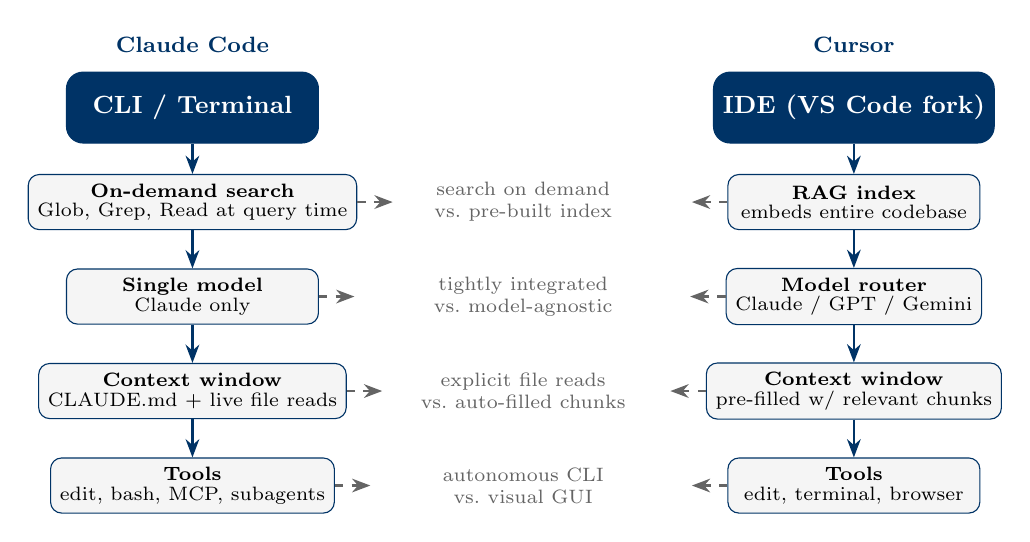
\begin{tikzpicture}[
  box/.style={draw=darkblue, rounded corners=4pt, fill=lightgray,
    minimum width=3.2cm, minimum height=0.7cm, align=center,
    font=\scriptsize},
  core/.style={draw=darkblue, rounded corners=6pt, fill=darkblue,
    text=white, minimum width=3.2cm, minimum height=0.9cm,
    align=center, font=\small\bfseries},
  lbl/.style={font=\footnotesize\bfseries, darkblue},
  arw/.style={-{Stealth}, thick, darkblue},
  dim/.style={-{Stealth}, thick, medgray, dashed},
]
% ---- Claude Code column (left) ----
\node[lbl] at (-4.2, 3.4) {Claude Code};
\node[core] (a-cli) at (-4.2, 2.6) {CLI / Terminal};
\node[box]  (a-search) at (-4.2, 1.4) {\textbf{On-demand search}\\[-1pt]
  Glob, Grep, Read at query time};
\node[box]  (a-mod) at (-4.2, 0.2) {\textbf{Single model}\\[-1pt]
  Claude only};
\node[box]  (a-ctx) at (-4.2,-1.0) {\textbf{Context window}\\[-1pt]
  CLAUDE.md + live file reads};
\node[box]  (a-tool) at (-4.2,-2.2) {\textbf{Tools}\\[-1pt]
  edit, bash, MCP, subagents};

\draw[arw] (a-cli) -- (a-search);
\draw[arw] (a-search) -- (a-mod);
\draw[arw] (a-mod) -- (a-ctx);
\draw[arw] (a-ctx) -- (a-tool);

% ---- Cursor column (right) ----
\node[lbl] at (4.2, 3.4) {Cursor};
\node[core] (c-ide) at (4.2, 2.6) {IDE (VS Code fork)};
\node[box]  (c-rag) at (4.2, 1.4) {\textbf{RAG index}\\[-1pt]
  embeds entire codebase};
\node[box]  (c-mod) at (4.2, 0.2) {\textbf{Model router}\\[-1pt]
  Claude / GPT / Gemini};
\node[box]  (c-ctx) at (4.2,-1.0) {\textbf{Context window}\\[-1pt]
  pre-filled w/ relevant chunks};
\node[box]  (c-tool) at (4.2,-2.2) {\textbf{Tools}\\[-1pt]
  edit, terminal, browser};

\draw[arw] (c-ide) -- (c-rag);
\draw[arw] (c-rag) -- (c-mod);
\draw[arw] (c-mod) -- (c-ctx);
\draw[arw] (c-ctx) -- (c-tool);

% ---- Contrast annotations (center) ----
\node[font=\scriptsize, align=center, text=medgray] at (0, 1.4)
  {search on demand\\vs.\ pre-built index};
\node[font=\scriptsize, align=center, text=medgray] at (0, 0.2)
  {tightly integrated\\vs.\ model-agnostic};
\node[font=\scriptsize, align=center, text=medgray] at (0,-1.0)
  {explicit file reads\\vs.\ auto-filled chunks};
\node[font=\scriptsize, align=center, text=medgray] at (0,-2.2)
  {autonomous CLI\\vs.\ visual GUI};

\draw[dim] (a-search.east) -- ++(0.45,0);
\draw[dim] (c-rag.west)   -- ++(-0.45,0);
\draw[dim] (a-mod.east)   -- ++(0.45,0);
\draw[dim] (c-mod.west)   -- ++(-0.45,0);
\draw[dim] (a-ctx.east)   -- ++(0.45,0);
\draw[dim] (c-ctx.west)   -- ++(-0.45,0);
\draw[dim] (a-tool.east)  -- ++(0.45,0);
\draw[dim] (c-tool.west)  -- ++(-0.45,0);

\end{tikzpicture}
\end{center}
\vspace{-0.2cm}
\begin{center}
\small
\textbf{Claude Code}: finds code \emphgold{when} you ask (explicit tool calls, always current)\\
\textbf{Cursor}: finds code \emphgold{before} you ask (semantic search over embeddings)
\end{center}
\end{frame}

% --- CLI Agents ----------------------------------------------------------------
\begin{frame}[shrink=5]{CLI Agents: The Power Tools}
\begin{center}
\footnotesize
\begin{tabular}{@{}p{2.5cm}p{3.5cm}p{3.5cm}p{3cm}@{}}
\toprule
& \textbf{Claude Code} & \textbf{OpenAI Codex} & \textbf{Gemini CLI} \\
\midrule
\textbf{Strengths} & Most mature harness; compacting, skills, subagents, MCP & Strong reasoning; cloud-sandboxed execution & Google ecosystem \\
\textbf{Price} & \$20/mo (Pro)\newline \$100/mo (Max 5x)\newline \$200/mo (Max 20x) & \$20/mo (Plus)\newline \$200/mo (Pro) & \$20/mo (AI Pro)\newline \$125/mo (AI Ultra) \\
\textbf{Best for} & Extended autonomous work & Budget-constrained users & \\
\bottomrule
\end{tabular}
\end{center}
\vspace{0.3cm}
\begin{itemize}
  \item Economics community split: 51\% Claude Code, 18\% Codex (Panjwani poll, March 2026)
  \item The landscape shifts fast --- this is the current state, not the permanent answer
  \item Skills and project files are \emphgold{portable} across tools
\end{itemize}
\sourceref{Mollick (2026); Panjwani (2026)}
\end{frame}

% --- Agent-Native IDEs ---------------------------------------------------------
\begin{frame}[shrink=27]{Agent-Native IDEs}
\begin{center}
\begin{tikzpicture}
  \node at (0,0) {\includegraphics[width=1.4cm,height=1.4cm,keepaspectratio]{images/cursor.png}};
  \node at (2.4,0) {\includegraphics[width=1.4cm,height=1.4cm,keepaspectratio]{images/vs_code.png}};
  \node at (4.8,0) {\includegraphics[width=1.4cm,height=1.4cm,keepaspectratio]{images/windsurf.png}};
  \node at (7.2,0) {\includegraphics[width=1.4cm,height=1.4cm,keepaspectratio]{images/zed.png}};
  \node at (9.6,0) {\includegraphics[width=1.4cm,height=1.4cm,keepaspectratio]{images/antigravity.png}};
\end{tikzpicture}
\end{center}
\vspace{0.1cm}
\small
\begin{itemize}
  \item \textbf{Where they shine}: iterative editing with visual feedback --- great for \emphgold{teaching materials}, \LaTeX{} papers, and code you want to review line-by-line
  \item \textbf{Model-agnostic}: Cursor lets you switch between Claude, GPT, Gemini mid-workflow\\
    \textcolor{medgray}{\scriptsize Golub (Northwestern): ``select Claude for coding, GPT for math-heavy proofs''}
  \item \textbf{Overleaf} $\rightarrow$ GitHub $\rightarrow$ Cursor pipeline for collaborative \LaTeX{} editing
  \item \textbf{The lines are blurring}: VS Code now has extensions for Claude Code, Codex, and Gemini --- all CLI agents run inside an IDE
  \item \textbf{Pricing}: Cursor: Hobby (free) / Pro (\$20/mo) / Ultra (\$200/mo); VS Code free (extensions bring the agent)
\end{itemize}
\vspace{0.1cm}
\begin{bigquote}
CLI agents and agentic IDEs \emphgold{complement} each other --- you can run Claude Code inside Cursor's terminal. Pick the right tool for the task, not the task for the tool.
\end{bigquote}
\sourceref{Golub (2025), Markus Academy; Mollick (2026)}
\end{frame}

% --- Additional Useful Tools ---------------------------------------------------
\begin{frame}{Additional Useful Tools}
\footnotesize
\renewcommand{\arraystretch}{1.4}
\begin{center}
\begin{tabular}{@{} l l p{7cm} @{}}
\toprule
\textbf{Tool} & \textbf{Cost} & \textbf{What It Does} \\
\midrule
GitHub Pro & Free / \$4 & Copilot included; essential for agentic workflows \\
refine.ink & Free preview & AI referee reports; finds math errors \& cross-paper inconsistencies \\
Whispr Flow & Free / \$8 & Voice-to-text dictation; built for \emphgold{prompting by voice} \\
Obsidian & Free & Local markdown knowledge base; \emphgold{wikilinks}, graph view, plugins \\
NotebookLM & Free / \$20 & Upload 300 papers; \emphgold{paragraph-level citations}; generates podcasts, videos, slides \\
Elicit & Free / paid & AI literature search; extracts claims, methods, findings \\
Perplexity & Free / \$20 & Web search with inline citations; quick fact-checking \\
\bottomrule
\end{tabular}
\end{center}
\renewcommand{\arraystretch}{1.0}
\end{frame}

% =============================================================================
\section{Claude Code: Practical Advice}
% =============================================================================

% --- The Claude Code Harness ---------------------------------------------------
\begin{frame}[shrink=15]{The Agentic Harness: Claude Code}
\begin{center}
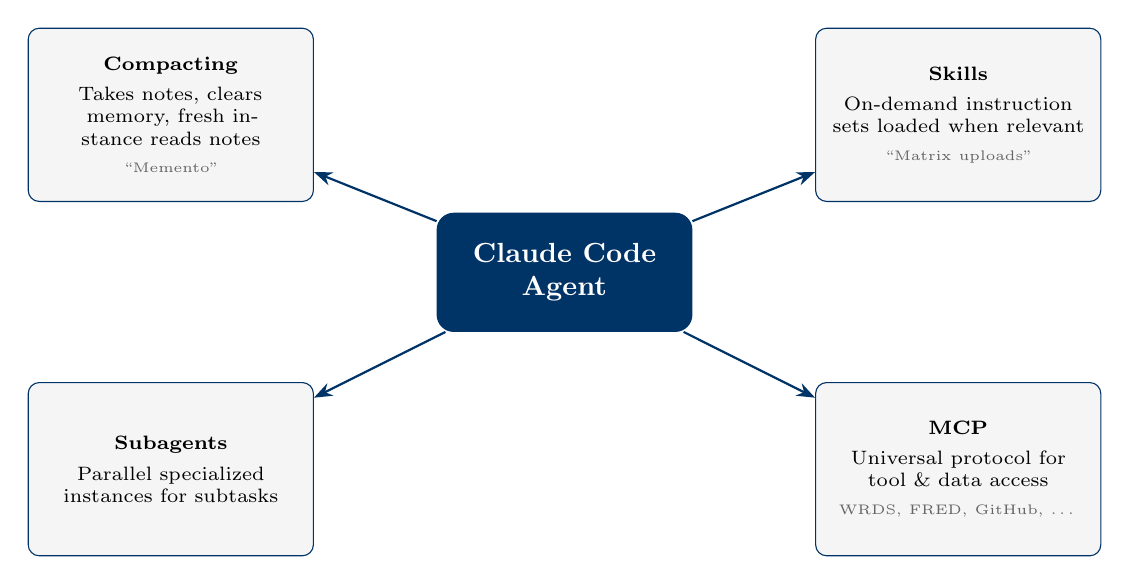
\begin{tikzpicture}[
  core/.style={draw=darkblue, rounded corners=6pt, fill=darkblue,
    text=white, text width=3cm, minimum height=1.5cm,
    align=center, font=\normalsize\bfseries},
  feat/.style={draw=darkblue, rounded corners=4pt, fill=lightgray,
    text width=3.2cm, minimum height=2.2cm, align=center,
    font=\scriptsize, inner sep=6pt},
  arw/.style={-{Stealth}, thick, darkblue},
]
\node[core] (cc) at (0,0) {Claude Code\\Agent};

\node[feat] (compact) at (-5,2) {\textbf{Compacting}\\[3pt]
  Takes notes, clears memory, fresh instance reads notes\\[2pt]
  \textcolor{medgray}{\tiny ``Memento''}};

\node[feat] (skills) at (5,2) {\textbf{Skills}\\[3pt]
  On-demand instruction sets loaded when relevant\\[2pt]
  \textcolor{medgray}{\tiny ``Matrix uploads''}};

\node[feat] (sub) at (-5,-2.5) {\textbf{Subagents}\\[3pt]
  Parallel specialized instances for subtasks};

\node[feat] (mcp) at (5,-2.5) {\textbf{MCP}\\[3pt]
  Universal protocol for tool \& data access\\[2pt]
  \textcolor{medgray}{\tiny WRDS, FRED, GitHub, \ldots}};

\draw[arw] (cc) -- (compact);
\draw[arw] (cc) -- (skills);
\draw[arw] (cc) -- (sub);
\draw[arw] (cc) -- (mcp);
\end{tikzpicture}
\end{center}
\sourceref{Mollick (2026), ``Claude Code and What Comes Next''}
\end{frame}

% --- CLAUDE.md Files -----------------------------------------------------------
\begin{frame}[fragile,shrink=31]{\texttt{CLAUDE.md} --- Teaching the Agent Your Rules}
\begin{columns}[T]
\column{0.48\textwidth}
\begin{keyinsight}[Project-Level \texttt{CLAUDE.md}]
Lives in the repo root. Loaded \emphgold{automatically} every session.
\begin{itemize}
  \item Defines what this project \emph{is} and how to work in it
  \item Rules, conventions, file structure --- set once
\end{itemize}
\end{keyinsight}
\vspace{0.1cm}
\begin{codeblock}
\scriptsize
\begin{verbatim}
# CLAUDE.md
## What This Project Is
Empirical asset pricing study.

## Rules
- All data pulled via WRDS API
- Use Python 3.12+, pandas, statsmodels
- Short variable names: ret, me, bm
- Compile LaTeX with latexmk
\end{verbatim}
\end{codeblock}

\column{0.48\textwidth}
\begin{keyinsight}[User-Level \texttt{\textasciitilde/.claude/CLAUDE.md}]
Personal preferences that follow you across \emphgold{all projects}.
\begin{itemize}
  \item Coding background, preferred stack, data sources
  \item Behavioral rules the agent always respects
\end{itemize}
\end{keyinsight}
\vspace{0.1cm}
\begin{codeblock}
\scriptsize
\begin{verbatim}
# Preferences
- Do not assume -- confirm with me.
- Make atomic git commits as you go.
- Explain Python idioms (MATLAB background)

# Data
- WRDS API (wrds package)
- Core datasets: CRSP, Compustat
\end{verbatim}
\end{codeblock}
\end{columns}
\vspace{0.15cm}
\begin{center}
\small The agent's behavior is shaped by \emphgold{persistent configuration}, not one-off prompts.
\end{center}
\end{frame}

% --- Plan Mode -----------------------------------------------------------------
\begin{frame}[shrink=26]{Plan Mode --- Think Before You Build}
\begin{columns}[T]
\column{0.52\textwidth}
\begin{keyinsight}[How Plan Mode Works]
\begin{enumerate}
  \item You describe the task
  \item Agent enters \emphgold{read-only} exploration
  \item Reads codebase, designs approach, identifies files to change
  \item Writes a \texttt{PLAN.md} --- persists even if context is compressed
  \item Presents the plan for your approval
  \item Only after you approve: editing begins
\end{enumerate}
\end{keyinsight}

\column{0.44\textwidth}
\begin{keyinsight}[Why This Matters]
\begin{itemize}
  \item Prevents wasted effort on the wrong approach
  \item \emphgold{Especially important for data pipelines} --- the cost of re-running is high
  \item You stay in control; the agent does the legwork
  \item Plans survive context compression --- the agent doesn't ``forget'' the approach mid-task
\end{itemize}
\end{keyinsight}
\end{columns}
\vspace{0.1cm}
\begin{bigquote}
Sant'Anna's ``plan-first workflow'': non-trivial tasks \emphgold{always} start in plan mode. The agent can't edit files until you approve the plan.
\end{bigquote}
\sourceref{Sant'Anna (2026), ``My Claude Code Setup''}
\end{frame}

% --- Skills --------------------------------------------------------------------
\begin{frame}[shrink=35]{Skills --- On-Demand Research Workflows}
\begin{keyinsight}[Slash Commands]
Instruction files in \texttt{.claude/skills/} --- loaded on demand when you type the command. Each defines a \emphgold{multi-step workflow} the agent executes autonomously.
\end{keyinsight}
\vspace{0.1cm}
\begin{columns}[T]
\column{0.48\textwidth}
\begin{keyinsight}[Research Skills (Sant'Anna)]
\begin{itemize}
  \item \texttt{/review-paper} --- manuscript review with adversarial critic-fixer loop
  \item \texttt{/data-analysis} --- end-to-end R/Python analysis pipeline
  \item \texttt{/lit-review} --- literature synthesis
  \item \texttt{/research-ideation} --- hypothesis generation
  \item \texttt{/interview-me} --- formalize ideas through structured Q\&A
\end{itemize}
\end{keyinsight}

\column{0.48\textwidth}
\begin{keyinsight}[10 Specialized Agents]
\scriptsize
\begin{itemize}
  \item Proofreader
  \item Slide auditor
  \item Pedagogy reviewer
  \item R code reviewer
  \item TikZ critic
  \item Domain reviewer
  \item Adversarial QA pair (critic + fixer)
  \item Translator
  \item Verifier
\end{itemize}
\end{keyinsight}
\end{columns}
\vspace{0.1cm}
\begin{center}
\small Skills turn \emphgold{recurring research workflows} into single commands. 22 slash commands + 18 context-aware rules. Adopted by 15+ research groups.
\end{center}
\sourceref{Sant'Anna (2026), ``My Claude Code Setup''}
\end{frame}

% --- Git Integration -----------------------------------------------------------
\begin{frame}[fragile,shrink=20]{Git Integration --- Reproducibility by Default}
\begin{columns}[T]
\column{0.48\textwidth}
\begin{keyinsight}[Git-Aware from Birth]
\begin{itemize}
  \item Claude Code reads your \emphgold{git history} to understand the project
  \item Creates branches, commits, and pull requests autonomously
  \item Every skill can end with a descriptive commit
  \item \emphgold{Every change is tracked} --- you can always revert
  \item Agentic IDEs (Cursor, Windsurf) have git integration \emphgold{built in}
\end{itemize}
\end{keyinsight}

\column{0.48\textwidth}
\begin{keyinsight}[Configure Git in CLAUDE.md]
\begin{codeblock}
\scriptsize
\begin{verbatim}
## Git Rules
- Atomic commits w/ descriptive msgs
- Never commit raw data files
- Format: "Add: <description>"
- Branch for each new analysis
\end{verbatim}
\end{codeblock}
\end{keyinsight}
\end{columns}
\vspace{0.2cm}
\begin{warningbox}[Why This Matters for Research]
Every data transformation, every analysis step gets a commit message explaining \emph{why}. Coauthors (and future you) can trace the full chain of reasoning. This is \emphgold{computational reproducibility} without extra effort.
\end{warningbox}
\end{frame}

% --- The Configuration Stack ---------------------------------------------------
\begin{frame}[shrink=10]{The Configuration Stack}
\begin{center}
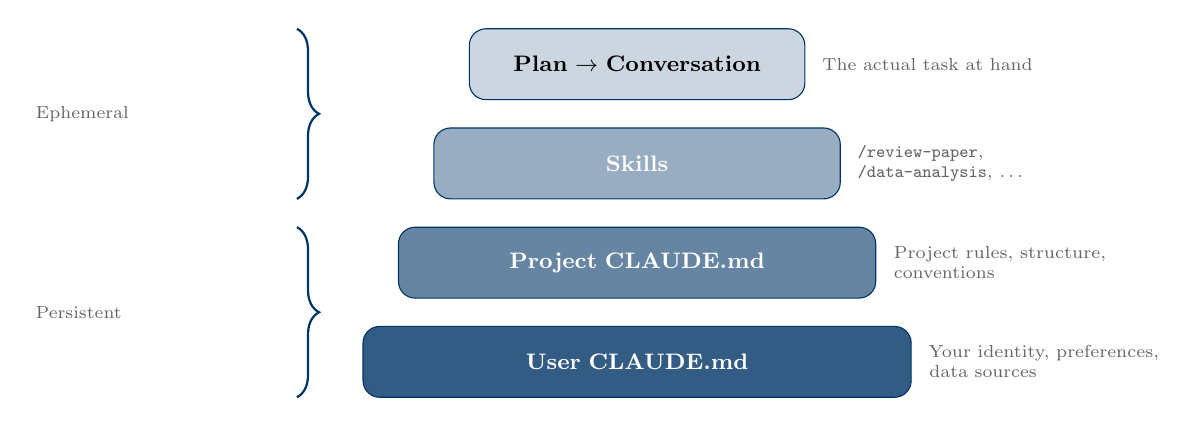
\begin{tikzpicture}[scale=0.9, every node/.style={transform shape},
  layer/.style={draw=darkblue, rounded corners=6pt, minimum height=1.0cm,
    align=center, font=\small},
  ann/.style={font=\scriptsize, text=medgray, align=left, text width=3.2cm},
]
% Stack layers (bottom to top, widest to narrowest)
\node[layer, fill=darkblue!80, text=white, text width=7.5cm]
  (user) at (0,0) {\textbf{User CLAUDE.md}};
\node[layer, fill=darkblue!60, text=white, text width=6.5cm]
  (proj) at (0,1.4) {\textbf{Project CLAUDE.md}};
\node[layer, fill=darkblue!40, text=white, text width=5.5cm]
  (skill) at (0,2.8) {\textbf{Skills}};
\node[layer, fill=darkblue!20, text width=4.5cm]
  (plan) at (0,4.2) {\textbf{Plan $\rightarrow$ Conversation}};

% Right-side annotations
\node[ann, right] at (4.0,0) {Your identity, preferences, data sources};
\node[ann, right] at (3.5,1.4) {Project rules, structure, conventions};
\node[ann, right] at (3.0,2.8) {\texttt{/review-paper}, \texttt{/data-analysis}, \ldots};
\node[ann, right] at (2.5,4.2) {The actual task at hand};

% Brace and label on the left
\draw[decorate, decoration={brace, amplitude=8pt, mirror}, thick, darkblue]
  (-4.8,-0.5) -- (-4.8,1.9) node[midway, left=10pt, ann] {Persistent};
\draw[decorate, decoration={brace, amplitude=8pt, mirror}, thick, darkblue]
  (-4.8,2.3) -- (-4.8,4.7) node[midway, left=10pt, ann] {Ephemeral};
\end{tikzpicture}
\end{center}
\vspace{0.1cm}
\begin{center}
\small Configure once, use everywhere. The agent improves as your \emphgold{project infractructure} gets better --- not as your prompts get longer.
\end{center}
\end{frame}


% =============================================================================
\section{Use Cases Across the Research Workflow}
% =============================================================================

% --- Research Pipeline overview (revised with Planning stage) ------------------
\begin{frame}[fragile]{The Research Pipeline}
\begin{center}
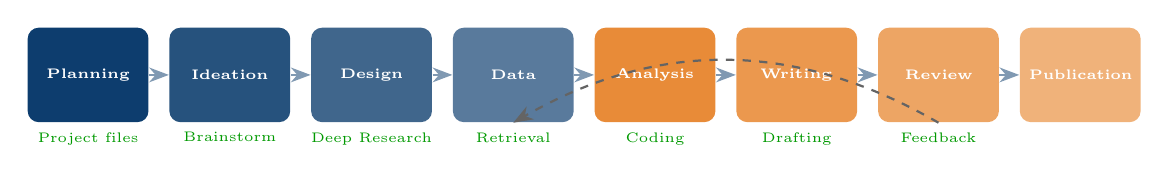
\begin{tikzpicture}[
  stage/.style={draw=none, rounded corners=4pt, fill=#1,
    text width=1.3cm, minimum height=1.2cm, align=center,
    font=\tiny\bfseries, text=white},
  arw/.style={-{Stealth[length=2.5mm]}, thick, darkblue!50},
]
\node[stage=darkblue!95] (s0) at (0,0) {Planning};
\node[stage=darkblue!85] (s1) at (1.8,0) {Ideation};
\node[stage=darkblue!75] (s2) at (3.6,0) {Design};
\node[stage=darkblue!65] (s3) at (5.4,0) {Data};
\node[stage=accentorange!90] (s4) at (7.2,0) {Analysis};
\node[stage=accentorange!80] (s5) at (9.0,0) {Writing};
\node[stage=accentorange!70] (s6) at (10.8,0) {Review};
\node[stage=accentorange!60] (s7) at (12.6,0) {Publication};

\draw[arw] (s0) -- (s1);
\draw[arw] (s1) -- (s2);
\draw[arw] (s2) -- (s3);
\draw[arw] (s3) -- (s4);
\draw[arw] (s4) -- (s5);
\draw[arw] (s5) -- (s6);
\draw[arw] (s6) -- (s7);

% Feedback arrow
\draw[arw, dashed, medgray] (s6.south) to[bend right=30] (s3.south);

% AI labels
\node[font=\tiny, text=sage, anchor=north] at (s0.south) {Project files};
\node[font=\tiny, text=sage, anchor=north] at (s1.south) {Brainstorm};
\node[font=\tiny, text=sage, anchor=north] at (s2.south) {Deep Research};
\node[font=\tiny, text=sage, anchor=north] at (s3.south) {Retrieval};
\node[font=\tiny, text=sage, anchor=north] at (s4.south) {Coding};
\node[font=\tiny, text=sage, anchor=north] at (s5.south) {Drafting};
\node[font=\tiny, text=sage, anchor=north] at (s6.south) {Feedback};
\end{tikzpicture}
\end{center}
\vspace{0.5cm}
\begin{columns}[T]
\column{0.48\textwidth}
\begin{keyinsight}[AI Replicates]
Execution skills: coding, data cleaning, drafting, formatting, literature search
\end{keyinsight}

\column{0.48\textwidth}
\begin{keyinsight}[Humans Provide]
Judgment skills: research taste, identification strategy, institutional knowledge
\end{keyinsight}
\end{columns}
\sourceref{Goldsmith-Pinkham (2025)}
\end{frame}

% --- Ideation: Karpathy's LLM Mirror ------------------------------------------
\begin{frame}[shrink=11]{Ideation: The LLM Mirror}
\vfill
\begin{bigquote}
\large
``Drafted a blog post. Used an LLM to meticulously improve the argument over 4 hours. Wow, feeling great, it's so convincing! Fun idea let's ask it to argue the opposite. LLM \emphgold{demolishes the entire argument} and convinces me that the opposite is in fact true. lol''
\end{bigquote}
\vspace{0.5cm}
\hfill\textcolor{medgray}{\normalsize --- Andrej Karpathy}
\vspace{0.5cm}
\begin{keyinsight}[LLMs as Devil's Advocate]
LLMs are trained to argue \emph{any} position persuasively. Use this deliberately: have the AI attack your own hypothesis before you invest months in a project.
\end{keyinsight}
\vfill
\sourceref{Karpathy (2026), X post}
\end{frame}

% --- Planning / Project Management ---------------------------------------------
\begin{frame}[shrink=19]{Planning: AI Project Folders}
\begin{columns}[T]
\column{0.50\textwidth}
\begin{keyinsight}[The Problem]
Every new AI conversation starts from scratch --- you re-explain your preferences, constraints, and context every time.
\end{keyinsight}
\vspace{0.3cm}
\textbf{The solution: project files}
\begin{enumerate}
  \item Dump everything about the domain
  \item Have AI interview you (preferences, avoids, thresholds)
  \item Synthesize into a canonical file ($<$500 words)
\end{enumerate}

\column{0.45\textwidth}
\begin{keyinsight}[Examples]
\begin{itemize}
  \item \textbf{CLAUDE.md}: project instructions loaded automatically by coding agents
  \item \textbf{ChatGPT Projects}: persistent context across conversations
  \item \textbf{Research folders}: lit review prefs, journal filters, methodology standards
\end{itemize}
\end{keyinsight}
\end{columns}
\vspace{0.3cm}
\begin{center}
\small Files develop through use, not upfront design. Failures teach the rules.
\end{center}
\sourceref{Blattman (2026), ``AI Project Folders''}
\end{frame}

% --- Design & Literature Review: Deep Research ---------------------------------
\begin{frame}[shrink=12]{Literature Review: Deep Research}
\begin{columns}[T]
\column{0.48\textwidth}
\begin{keyinsight}[What It Does]
\begin{itemize}
  \item Multi-agent architecture searches \emphgold{hundreds of sources} in 5--30 minutes
  \item Compiles structured reports with citations
  \item Maps literature landscapes, identifies gaps
  \item ``Potentially the single most valuable AI tool for faculty'' --- Blattman
\end{itemize}
\end{keyinsight}

\column{0.48\textwidth}
\begin{warningbox}[Handle with Care]
\begin{itemize}
  \item May confidently cite \emphgold{unreliable sources}
  \item Sometimes \emphgold{fabricates} references entirely
  \item Best used as starting point, not final product
  \item Always verify citations against actual sources
\end{itemize}
\end{warningbox}
\end{columns}
\vspace{0.3cm}
\begin{center}
\small Available in ChatGPT (Deep Research), Claude (research mode), Gemini (Deep Research).
\end{center}
\sourceref{Korinek (2025); Blattman (2026)}
\end{frame}

% --- Data Collection: WRDS via Claude Code --------------------------------------
\begin{frame}[shrink=14]{Data Collection: Claude Code WRDS Toolkit}
\begin{columns}[T]
\column{0.48\textwidth}
\begin{keyinsight}[Specialist Agents (Orlowski)]
\begin{itemize}
  \item \texttt{crsp-wrds-expert} --- stock returns
  \item \texttt{optionmetrics-wrds-expert} --- options
  \item \texttt{taq-wrds-expert} --- high-frequency
  \item \texttt{wrds-query-orchestrator} --- cross-database merges (link tables built in)
\end{itemize}
\end{keyinsight}

\column{0.48\textwidth}
\begin{keyinsight}[How It Works]
\begin{itemize}
  \item Describe data in \emphgold{natural language}
  \item Agent picks the right database, schema, and link tables
  \item Skills pre-load schemas to avoid exploratory round-trips
  \item TAQ handled via SSH + SAS batch jobs on the WRDS grid
\end{itemize}
\end{keyinsight}
\end{columns}
\vspace{0.5cm}
\begin{center}
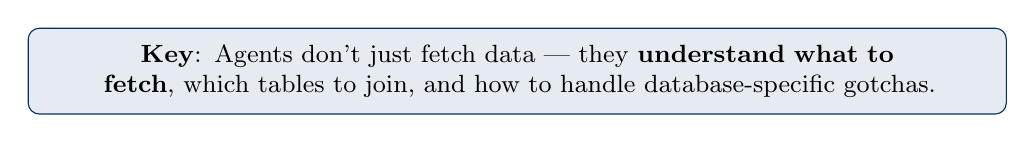
\begin{tikzpicture}
\node[draw=darkblue, rounded corners, fill=darkblue!10, inner sep=6pt,
  font=\small, text width=12cm, align=center] {%
  \textbf{Key}: Agents don't just fetch data --- they \emphgold{understand what to fetch},
  which tables to join, and how to handle database-specific gotchas.
};
\end{tikzpicture}
\end{center}
\sourceref{\href{https://github.com/piotrek-orlowski/claude-wrds-public}{Orlowski (2026), Claude Code WRDS Toolkit}}
\end{frame}

% --- Data Collection: Empty Folder to Figure (moved from Section 3) ------------
\begin{frame}[shrink=16]{Data Collection: Empty Folder to Figure}
\begin{keyinsight}[Goldsmith-Pinkham --- ``How has the age distribution of homeowners changed over 50 years?'']
A deliberately \emphgold{vague} prompt to Claude Code in a brand-new directory.
\end{keyinsight}
\vspace{0.3cm}
\begin{columns}[T]
\column{0.50\textwidth}
\textbf{What the agent did autonomously:}
\begin{enumerate}
  \item Tried FRED first --- hit a dead end
  \item Switched to Census Bureau website
  \item Got 403 error --- added user-agent header to bypass bot-blocking
  \item Found \emph{two} relevant tables with different tradeoffs
  \item Decided to pull \emph{both}
  \item Parsed messy government Excel files
  \item Produced two clean CSVs
\end{enumerate}

\column{0.45\textwidth}
\vspace{0.3cm}
\begin{center}
\textbf{Timeline:} \emphgold{6 minutes, 21 seconds}
\end{center}
\vspace{0.3cm}
\begin{itemize}
  \item Agent made \emph{real decisions}
  \item Recovered from dead ends
  \item ``It's exactly what you'd want an RA to do''
  \item Spawned a \textbf{sub-agent} for web research (context management)
\end{itemize}
\end{columns}
\sourceref{Goldsmith-Pinkham (2026), Markus Academy}
\end{frame}

% --- Data Collection: Iteration (moved from Section 3) -------------------------
\begin{frame}[shrink=6]{Data Collection: Iteration}
\begin{columns}[T]
\column{0.50\textwidth}
\textbf{The prompt trick:}
\begin{codeblock}
\small
``Please make a figure in R. Follow the best practices of \emphgold{Kieran Healy}.''
\end{codeblock}
\vspace{0.1cm}
\begin{itemize}
  \item Claude translates this into: clean ggplot2, direct labeling, minimal chart junk, thoughtful color
  \item First version: broad age buckets (not what was needed)
  \item User iterates: ``I want age on x-axis with different lines for each year''
  \item Agent re-fetches finer data, regenerates, auto-fixes overlapping labels
\end{itemize}

\column{0.45\textwidth}
\vspace{0.3cm}
\begin{keyinsight}[Key Lessons]
\begin{itemize}
  \item \emphgold{Iteration} is fast and natural
  \item ``What would take an hour of ggplot2 fiddling took three rounds of conversation''
  \item Agent is like a good RA: tries to make nice graphs, catches straightforward issues
  \item Human decides \emph{what story matters}
\end{itemize}
\end{keyinsight}
\end{columns}
\sourceref{Goldsmith-Pinkham (2026)}
\end{frame}

% --- Data Collection: EDGAR before/after ---------------------------------------
\begin{frame}[shrink=3]{Data Collection: EDGAR Example}
\begin{columns}[T]
\column{0.48\textwidth}
\begin{warningbox}[Before: Manual Pipeline]
\begin{enumerate}
  \item Write custom scraper
  \item Parse HTML/XML filings
  \item Handle edge cases manually
  \item Debug encoding issues
  \item Weeks of work
\end{enumerate}
\end{warningbox}

\column{0.48\textwidth}
\begin{keyinsight}[After: Agent-Assisted]
\begin{enumerate}
  \item Describe what you need in plain English
  \item Agent writes scraper + parser
  \item Agent handles edge cases
  \item Agent tests and debugs
  \item Hours, not weeks
\end{enumerate}
\end{keyinsight}
\end{columns}
\vspace{0.5cm}
\begin{center}
\small AI replicates the \emphgold{execution} (scraping, parsing) --- human provides the \emphgold{judgment} (what to extract, why it matters).
\end{center}
\sourceref{Goldsmith-Pinkham (2025)}
\end{frame}


% --- Writing: Voice files -----------------------------------------------------
\begin{frame}[shrink=5]{Writing: Teaching AI Your Voice}
\begin{columns}[T]
\column{0.48\textwidth}
\begin{warningbox}[Before: AI Default Style]
\begin{itemize}
  \item Generic, corporate tone
  \item ``Furthermore\ldots'' ``Delve into\ldots''
  \item ``Robust and compelling\ldots''
  \item Sounds like \emph{every} AI output
\end{itemize}
\end{warningbox}

\column{0.48\textwidth}
\begin{keyinsight}[After: Voice File]
\begin{itemize}
  \item 5--10 writing samples analyzed
  \item AI generates style guide
  \item \emphgold{Annotated examples} beat abstract rules
  \item Add a ``ban list'' of AI-isms
\end{itemize}
\end{keyinsight}
\end{columns}
\vspace{0.5cm}
\begin{bigquote}
\small
The voice file approach: collect samples $\rightarrow$ analyze patterns $\rightarrow$ generate style spec $\rightarrow$ add annotated examples $\rightarrow$ maintain a ban list.
\end{bigquote}
\sourceref{Blattman (2025), ``Teaching AI Your Voice''}
\end{frame}

% --- Review: refine.ink -------------------------------------------------------
\begin{frame}[shrink=17]{Review: AI Referee Reports}
\begin{columns}[T]
\column{0.48\textwidth}
\begin{keyinsight}[refine.ink]
\begin{itemize}
  \item Founded by \textbf{Benjamin Golub} (Northwestern) \& \textbf{Yann Calv\'{o} L\'{o}pez}
  \item Generates deep technical referee reports
  \item Detects \emphgold{cross-paper inconsistencies} (e.g., definition on p.~3 used incompatibly on p.~42)
  \item Finds subtle \emphgold{mathematical errors} (sign errors, logical gaps in proofs)
\end{itemize}
\end{keyinsight}

\column{0.48\textwidth}
\begin{keyinsight}[Why Now?]
\begin{itemize}
  \item AI-accelerated research makes quality control \emphgold{more} important, not less
  \item Strongest on theory papers; works for empirical too
  \item Ironclad privacy: papers never shared or used for training
  \item Several journals piloting as complement to peer review
\end{itemize}
\end{keyinsight}
\end{columns}
\vspace{0.15cm}
\begin{center}
\small Free preview: 10 comments per paper. Upload TeX source for best results.
\end{center}
\sourceref{Golub (2025), Markus Academy Ep.~154}
\end{frame}

% =============================================================================
% FULL AUTOMATED PIPELINES
% =============================================================================


% --- Gregoire: Vibe Research ---------------------------------------------------
\begin{frame}[shrink=6]{Full Pipeline: Vibe Research}
\begin{keyinsight}[Vincent Gregoire --- ``Investing in AGI'']
\begin{itemize}
  \item Idea from podcast $\rightarrow$ posted working paper in \emphgold{4 days}
  \item Workflow: Claude outline $\rightarrow$ Claude Code overnight draft $\rightarrow$ multi-agent review loops $\rightarrow$ iterative refinement
  \item Tools: Quarto, Python, Git/GitHub
  \item Multi-agent review: Claude Code + Codex CLI + Gemini
\end{itemize}
\end{keyinsight}
\vspace{0.3cm}
\begin{columns}[T]
\column{0.48\textwidth}
\begin{itemize}
  \item Caught 1 fabricated reference
  \item Caught 1 metadata error
  \item Human judgment still critical for idea selection, model steering
\end{itemize}

\column{0.48\textwidth}
\begin{bigquote}
\small
``Faster, not smarter'' --- AI accelerated execution but didn't substitute for research taste.
\end{bigquote}
\end{columns}
\sourceref{Gregoire (2025)}
\end{frame}


% --- Project APE ---------------------------------------------------------------
\begin{frame}[shrink=5]{Full Pipeline: Project APE}
\begin{keyinsight}[Automated Policy Evaluation]
\begin{itemize}
  \item David Yanagizawa-Drott's platform for \emphgold{fully automated} empirical policy evaluation
  \item Input: a policy question
  \item Output: complete empirical paper with identification, estimation, and interpretation
  \item 592 papers generated as of March 2026
\end{itemize}
\end{keyinsight}
\vspace{0.3cm}
\begin{columns}[T]
\column{0.48\textwidth}
\textbf{What it demonstrates:}
\begin{itemize}
  \item End-to-end research automation is here
  \item AI can handle data $\rightarrow$ estimation $\rightarrow$ writing
\end{itemize}

\column{0.48\textwidth}
\textbf{What it reveals:}
\begin{itemize}
  \item 64.2\% default to DiD
  \item Methodological monoculture risk
  \item More on this shortly\ldots
\end{itemize}
\end{columns}
\sourceref{Goldsmith-Pinkham (2026)}
\end{frame}

% --- Lopez-Lira: Automated Finance Papers --------------------------------------
\begin{frame}[shrink=5]{Full Pipeline: Automated Finance Papers}
\begin{keyinsight}[Lopez-Lira --- Automated Finance Papers]
Fully automated pipeline producing \emphgold{submission-ready finance papers in $\sim$1 day}.
\end{keyinsight}
\vspace{0.3cm}
\begin{center}
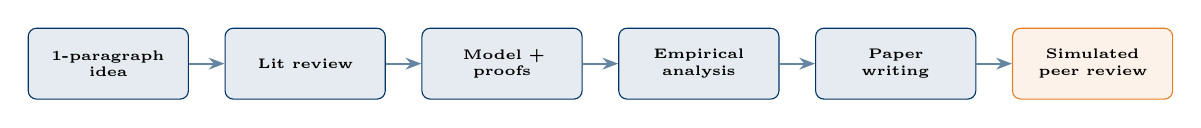
\begin{tikzpicture}[
  stp/.style={draw=darkblue, rounded corners=3pt, fill=darkblue!10,
    text width=1.8cm, minimum height=0.9cm, align=center, font=\tiny\bfseries},
  arw/.style={-{Stealth[length=2mm]}, thick, darkblue!60},
]
\node[stp] (s1) at (0,0) {1-paragraph\\idea};
\node[stp] (s2) at (2.5,0) {Lit review};
\node[stp] (s3) at (5,0) {Model +\\proofs};
\node[stp] (s4) at (7.5,0) {Empirical\\analysis};
\node[stp] (s5) at (10,0) {Paper\\writing};
\node[stp, draw=accentorange, fill=accentorange!10] (s6) at (12.5,0) {Simulated\\peer review};
\draw[arw] (s1) -- (s2);
\draw[arw] (s2) -- (s3);
\draw[arw] (s3) -- (s4);
\draw[arw] (s4) -- (s5);
\draw[arw] (s5) -- (s6);
\end{tikzpicture}
\end{center}
\vspace{0.3cm}
\begin{columns}[T]
\column{0.48\textwidth}
\begin{itemize}
  \item Data: WRDS (CRSP, Compustat, TAQ), FRED
  \item Quality gates at each stage
  \item Handles theory, empirical, or both
\end{itemize}

\column{0.48\textwidth}
\begin{itemize}
  \item Target quality: $\sim$JFQA level
  \item Goal: published papers + meta-paper on the process itself
\end{itemize}
\end{columns}
\sourceref{Lopez-Lira (2025)}
\end{frame}


% --- Quality control: Gans lessons --------------------------------------------
\begin{frame}{Quality Control: Lessons from Vibe Research}
\begin{columns}[T]
\column{0.48\textwidth}
\begin{warningbox}[Joshua Gans --- 3 Pitfalls]
\begin{enumerate}
  \item \textbf{Subtle errors}: AI gets equilibrium concepts wrong --- beyond simple math mistakes
  \item \textbf{Idea inflation}: lower costs $\rightarrow$ pursuing weaker ideas
  \item \textbf{Seductiveness}: confident results that are wrong
\end{enumerate}
\end{warningbox}

\column{0.48\textwidth}
\begin{keyinsight}[Guardrails]
\begin{itemize}
  \item \emphgold{Cooling-off period} (1+ month)
  \item More peer feedback
  \item Explicit go/no-go decisions
  \item Human taste matters \emph{more} than ever
\end{itemize}
\end{keyinsight}
\end{columns}
\vspace{0.2cm}
\begin{center}
\small\textcolor{darkblue}{\textbf{High-speed, low-human-input research did not produce high-quality output.}}
\end{center}
\sourceref{Gans (2026)}
\end{frame}

% =============================================================================
% DEMO SLOT (time permitting)
% =============================================================================

% =============================================================================
\section{Implications \& Getting Started}
% =============================================================================


% --- The Jagged Frontier -------------------------------------------------------
\begin{frame}[shrink=5]{The Jagged Frontier}
\small
\begin{bigquote}
``Shockingly capable at some hard things, embarrassingly bad at seemingly simple things.''
\hfill\textcolor{medgray}{\scriptsize --- Ethan Mollick, Wharton}
\end{bigquote}
\vspace{-0.2cm}
\begin{center}
\includegraphics[width=0.9\linewidth, height=0.6\textheight, keepaspectratio]{./images/jaggedFrontier.jpg}
\end{center}
\sourceref{Mollick et al.\ (2023)}
\end{frame}


% --- Key Takeaways -------------------------------------------------------------
\begin{frame}{Key Takeaways}
\begin{enumerate}
  \item \textbf{The shift is real} --- academic researchers are already transforming their workflows
  \item \textbf{Agents $>$ chatbots} --- autonomous tool use, planning, and multi-step execution
  \item \textbf{The harness matters more than the model} --- choose tools, not just AI brands
  \item \textbf{Exponential progress} --- task complexity doubling every 4--7 months
  \item \textbf{The hard part remains human} --- research taste, identification, institutional knowledge
  \item \textbf{Start now, start small} --- \$20/mo gets you in the door
\end{enumerate}
\vspace{0.3cm}
\begin{bigquote}
\large
``AI is a flashlight in the dark --- the hard part is still knowing where to walk.''
\hfill\textcolor{medgray}{\normalsize --- Goldsmith-Pinkham}
\end{bigquote}
\end{frame}

% --- Quick and Easy: Try This Today ---------------------------------------------
\begin{frame}[shrink=24]{Quick \& Easy --- Try This Today}
\begin{keyinsight}[Low-Risk, High-Reward First Projects]
You don't need a greenfield project. Point an agent at something you \emphgold{already have}.
\end{keyinsight}
\vspace{0.1cm}
\begin{columns}[T]
\column{0.48\textwidth}
\begin{enumerate}
  \item \textbf{Reorganize a messy repo}\\
    \textcolor{medgray}{\tiny Cunningham: ``use a coding agent to clean up, refactor, and reorganize existing project directories, with Git for safety and rollback''}
  \item \textbf{Make slides from a paper}\\
    \textcolor{medgray}{\tiny Feed it a PDF $\rightarrow$ get a Beamer or PowerPoint deck. Edit from there.}
  \item \textbf{Write a paper from a codebase}\\
    \textcolor{medgray}{\tiny Point it at your analysis scripts $\rightarrow$ get a first draft describing data, methods, and results.}
\end{enumerate}

\column{0.48\textwidth}
\begin{enumerate}
  \setcounter{enumi}{3}
  \item \textbf{Create a voice file}\\
    \textcolor{medgray}{\tiny Give it 5--10 writing samples $\rightarrow$ it generates a style guide for future drafts.}
  \item \textbf{Get an AI referee report}\\
    \textcolor{medgray}{\tiny Upload a working paper to refine.ink or use Sant'Anna's \texttt{/review-paper} skill.}
  \item \textbf{Translate code across languages}\\
    \textcolor{medgray}{\tiny Stata $\rightarrow$ R $\rightarrow$ Python. Cross-language replication catches errors.}
\end{enumerate}
\end{columns}
\vspace{0.15cm}
\begin{bigquote}
All six work with a \emphgold{\$20/month} subscription. Start with what you already have --- the agent meets you where you are.
\end{bigquote}
\sourceref{Cunningham (2026); Blattman (2025); Panjwani (2026)}
\end{frame}

% --- Who to Follow on X ---------------------------------------------------------
\begin{frame}{Economists to Follow on X on Agentic Coding}
\begin{columns}[T]
\column{0.48\textwidth}
\begin{itemize}
  \item Alex Imas: \texttt{@alexolegimas}
  \item Chris Blattman: \texttt{@cblatts}
  \item David Yanagizawa-Drott: \texttt{@YanagizawaD}
  \item Ethan Mollick: \texttt{@emollick}
  \item Kevin Bryan: \texttt{@Afinetheorem}
  \item Alexander Kustov: \texttt{@akoustov}
  \item Antonio Mele: \texttt{@antoniomele101}
\end{itemize}

\column{0.48\textwidth}
\begin{itemize}
  \item Anthony Lee Zhang: \texttt{@alz\_zyd\_}
  \item Aniket Panjwani: \texttt{@aniketapanjwani}
  \item Scott Cunningham: \texttt{@causalinf}
  \item Pedro Sant'Anna: \texttt{@pedrohcgs}
  \item Joshua Gans: \texttt{@joshgans}
  \item Jason Bell: \texttt{@j\_jason\_bell}
  \item Mihail Velikov: \texttt{@velikovmihail}
\end{itemize}
\end{columns}
\vspace{0.5cm}
\begin{center}
\small\textcolor{medgray}{Adapted from Panjwani (2026). Also follow the AI developers: \texttt{@dylan522p}, \texttt{@birchwork}, \texttt{@vanhoornm}.}
\end{center}
\end{frame}

% --- Resources ------------------------------------------------------------------
\begin{frame}[shrink=5]{Resources}
\begin{columns}[T]
\column{0.48\textwidth}
\begin{keyinsight}[Blogs \& Guides]
\begin{itemize}
  \item \textbf{Korinek}: \href{https://genaiforecon.org}{genaiforecon.org}
  \item \textbf{Mollick}: \href{https://oneusefulthing.org}{oneusefulthing.org}
  \item \textbf{Blattman}: \href{https://claudeblattman.com}{claudeblattman.com}
  \item \textbf{Cunningham}: \href{https://causalinf.substack.com}{causalinf.substack.com}
  \item \textbf{Goldsmith-Pinkham}: \href{https://paulgp.substack.com}{paulgp.substack.com}
  \item \textbf{Panjwani}: \href{https://aniketpanjwani.com/}{aniketpanjwani.com}
  \item \textbf{Sant'Anna}: \href{https://psantanna.com/claude-code-my-workflow/}{Claude Code workflow}
\end{itemize}
\end{keyinsight}

\column{0.48\textwidth}
\begin{keyinsight}[This Presentation's Wiki]
\begin{itemize}
  \item \href{https://velikov-mihail.github.io/ai-econ-wiki/}{velikov-mihail.github.io/ai-econ-wiki}
\end{itemize}
\end{keyinsight}
\end{columns}
\end{frame}

% --- Live Demo ------------------------------------------------------------------
\begin{frame}{Live Demo: Claude Code}
\vfill
\begin{center}
{\LARGE\bfseries\textcolor{darkblue}{Let's see an agent work in real time.}}
\end{center}
\vspace{1cm}
\begin{center}
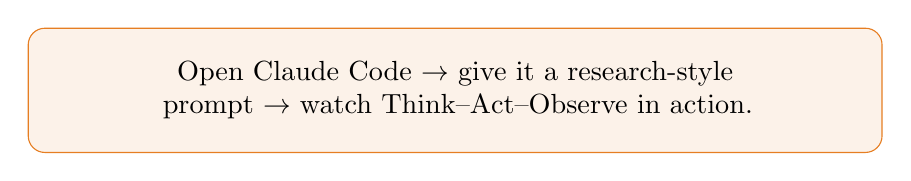
\begin{tikzpicture}
\node[draw=accentorange, rounded corners=6pt, fill=accentorange!10,
  text width=10cm, align=center, inner sep=12pt, font=\normalsize] {%
  Open Claude Code $\rightarrow$ give it a research-style prompt $\rightarrow$ watch Think--Act--Observe in action.
};
\end{tikzpicture}
\end{center}
\vfill
\end{frame}

% --- Thank You -------------------------------------------------------------------
\begin{frame}{}
\vfill
\begin{center}
{\large\bfseries\textcolor{darkblue}{Thank you!}}\\[0.5cm]
\textcolor{medgray}{Mihail Velikov --- velikov@psu.edu}
\end{center}
\vspace{1cm}
\begin{bigquote}
\large
``Holy crap.''
\hfill\textcolor{medgray}{\normalsize --- Chris Blattman, upon first using Claude Code}
\end{bigquote}
\vfill
\end{frame}

\end{document}
